\documentclass[addpoints]{exam}
% \documentclass[addpoints,12pt]{exam}

\usepackage[slovene]{babel}
\usepackage{amsfonts}
\usepackage{amssymb}
\usepackage{amsmath}
\usepackage{float}
\usepackage{graphicx}
\usepackage{enumitem}
\usepackage{color}
\usepackage{eurosym}

\usepackage{pgfpages}
% \usepackage{tikz}
\usepackage{wrapfig}
\usepackage{pgfkeys}
\usepackage{pgfplots}
\usepackage{xcolor}
\usepackage{tkz-euclide}
\usepackage{xfp}




%Komentar naslednje vrstice glede na verzijo testa -- rešitve ali prostor za odgovore:
% \printanswers

% \linespread{2}


\pointsinrightmargin
\marginbonuspointname{}


\renewcommand{\solutiontitle}{\noindent\textbf{Rešitve in točkovanje:}\par\noindent}

\colorgrids
\definecolor{GridColor}{gray}{0.7}
\setlength{\gridsize}{7mm}

\extrawidth{5mm}
\setlength{\rightpointsmargin}{1.5cm}

\begin{document}

\runningfooter{}{}{}

\begin{center}
    \fbox{\fbox{\parbox{15cm}{\centering
    Tretje pisno ocenjevanje znanja -- ponovno \\ 2. letnik -- test B \\ 26. marec 2026 \\ (Potence in koreni; Funkcija; Potenčna funkcija; Korenska funkcija)}}}
\end{center}

\vspace{0.1in}
\makebox[\textwidth]{Ime in priimek, oddelek:\enspace\hrulefill}


\begin{center}
    \chqword{Naloga}
    \chpword{Možne točke}
    \chbpword{Dodatne točke}
    \chsword{Dosežene točke}
    \chtword{Skupaj}  
    % \combinedpointtable[h][questions]
    \combinedgradetable[h][questions]

\end{center}

\vspace{0.1in}


\begin{questions}

    % 1. vprašanje

    \question[7]
    Izračunajte natančno vrednost izraza. 
    $$ \sqrt{\left(\frac{4}{9}\right)^{-0.5}\cdot 32^{0.2}+169^\frac{1}{2}} -\left(3-\sqrt{5}\right)\sqrt{7+3\sqrt{5}} $$

    \begin{solution}[7.5cm]
       
    \end{solution}


    % 2. vprašanje

    \question[6]
    Rešite enačbo. 
    $$ \sqrt{9+\sqrt{2x-1}-x~} = \sqrt{7} $$

    \begin{solution}[5.25cm]
       
    \end{solution}


\newpage
    % 3. vprašanje

    \question
    Dana je funkcija $f(x)=\sqrt{x+3}-2$.

    \begin{parts}
        \part[2]
        Zapišite definicijsko območje $D_f$ in zalogo vrednosti $Z_f$ funkcije $f$. 

            \begin{solution}[2cm]

            \end{solution}
        
        \part[3] 
        Izračunajte ničle in začetno vrednost funkcije $f$.
    
            \begin{solution}[5cm]

            \end{solution}

        \part[2] 
        Ali je funkcija $f$ soda ali liha? Utemeljite.
    
            \begin{solution}[4cm]

            \end{solution}

        \part[2]
        Zapišite predpis funkcije $g(x)=-3f(x-3)-6$. 

            \begin{solution}[2cm]

            \end{solution}


        \bonuspart[4] 
        \textit{Dodatna naloga:}  Določite presečišča grafa funkcije $f$ s premico $y=\frac{1}{4}x-\frac{1}{2}$.
    
            \begin{solution}[5cm]

            \end{solution}

        \newpage
        \part[4] 
        Narišite graf funkcije $f$.
    
            \begin{solution}[5cm]

            \end{solution}
            
    \end{parts}


    

    \newpage
    % 4. vprašanje

    \question
    Na sliki je graf funkcije $g$, ki smo ga dobili s transformacijo grafa funkcije $f(x)=x^2$.
    
    \begin{figure}[H]
        \centering
        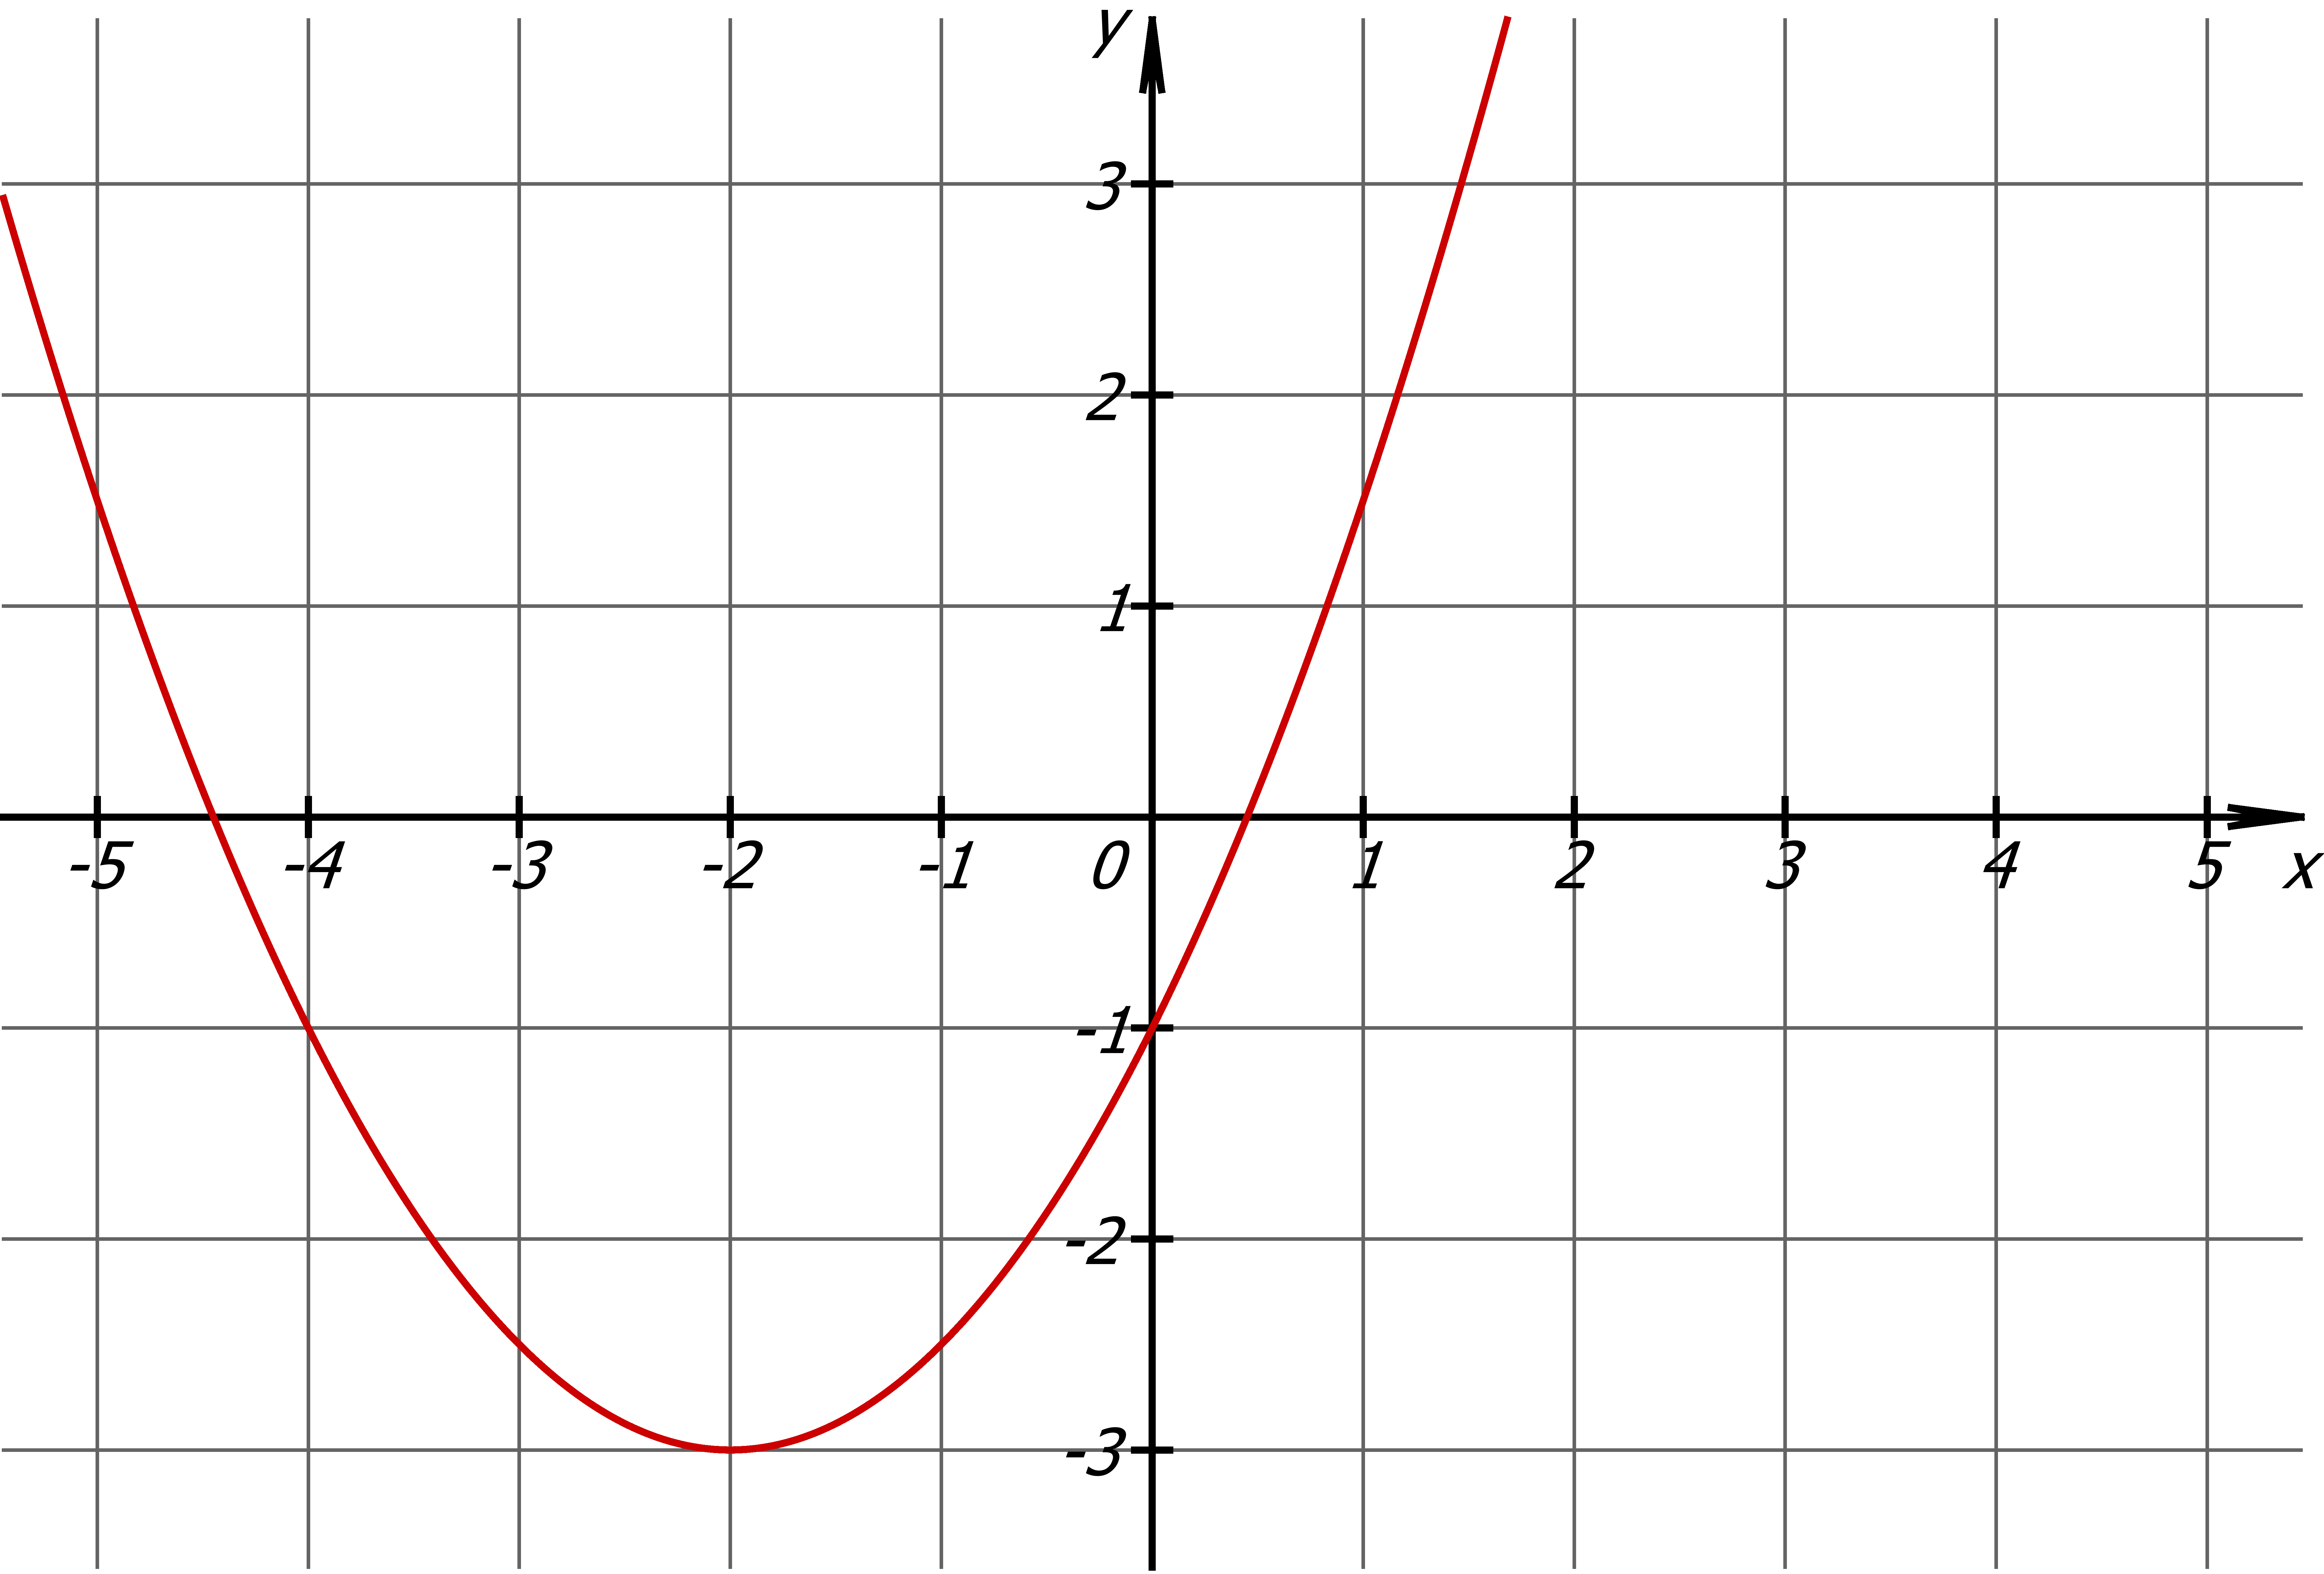
\includegraphics[scale=0.05]{test3_kvadratna.png}
    \end{figure}

    \begin{parts}
        \part[3] 
        Na zgornjo sliko dorišite graf funkcije $h(x)=\lvert g(x-4)\rvert$.
        
            \begin{solution}

            \end{solution}        

        \part[4]
        Zapišite predpis funkcije $g$, če njen graf poteka skozi točko $(2,5)$.

            \begin{solution}[7cm]

            \end{solution}

    
        \part[4]
        Določite inverzno funkcijo $l^{-1}$ funkciji $l(x)=-2 f(x+3) - 5$.
        
            \begin{solution}[5cm]

            \end{solution}


    \end{parts}





\end{questions}



\end{document}